\chapter{Server Side}
\begin{figure}[!ht]
  \centering
  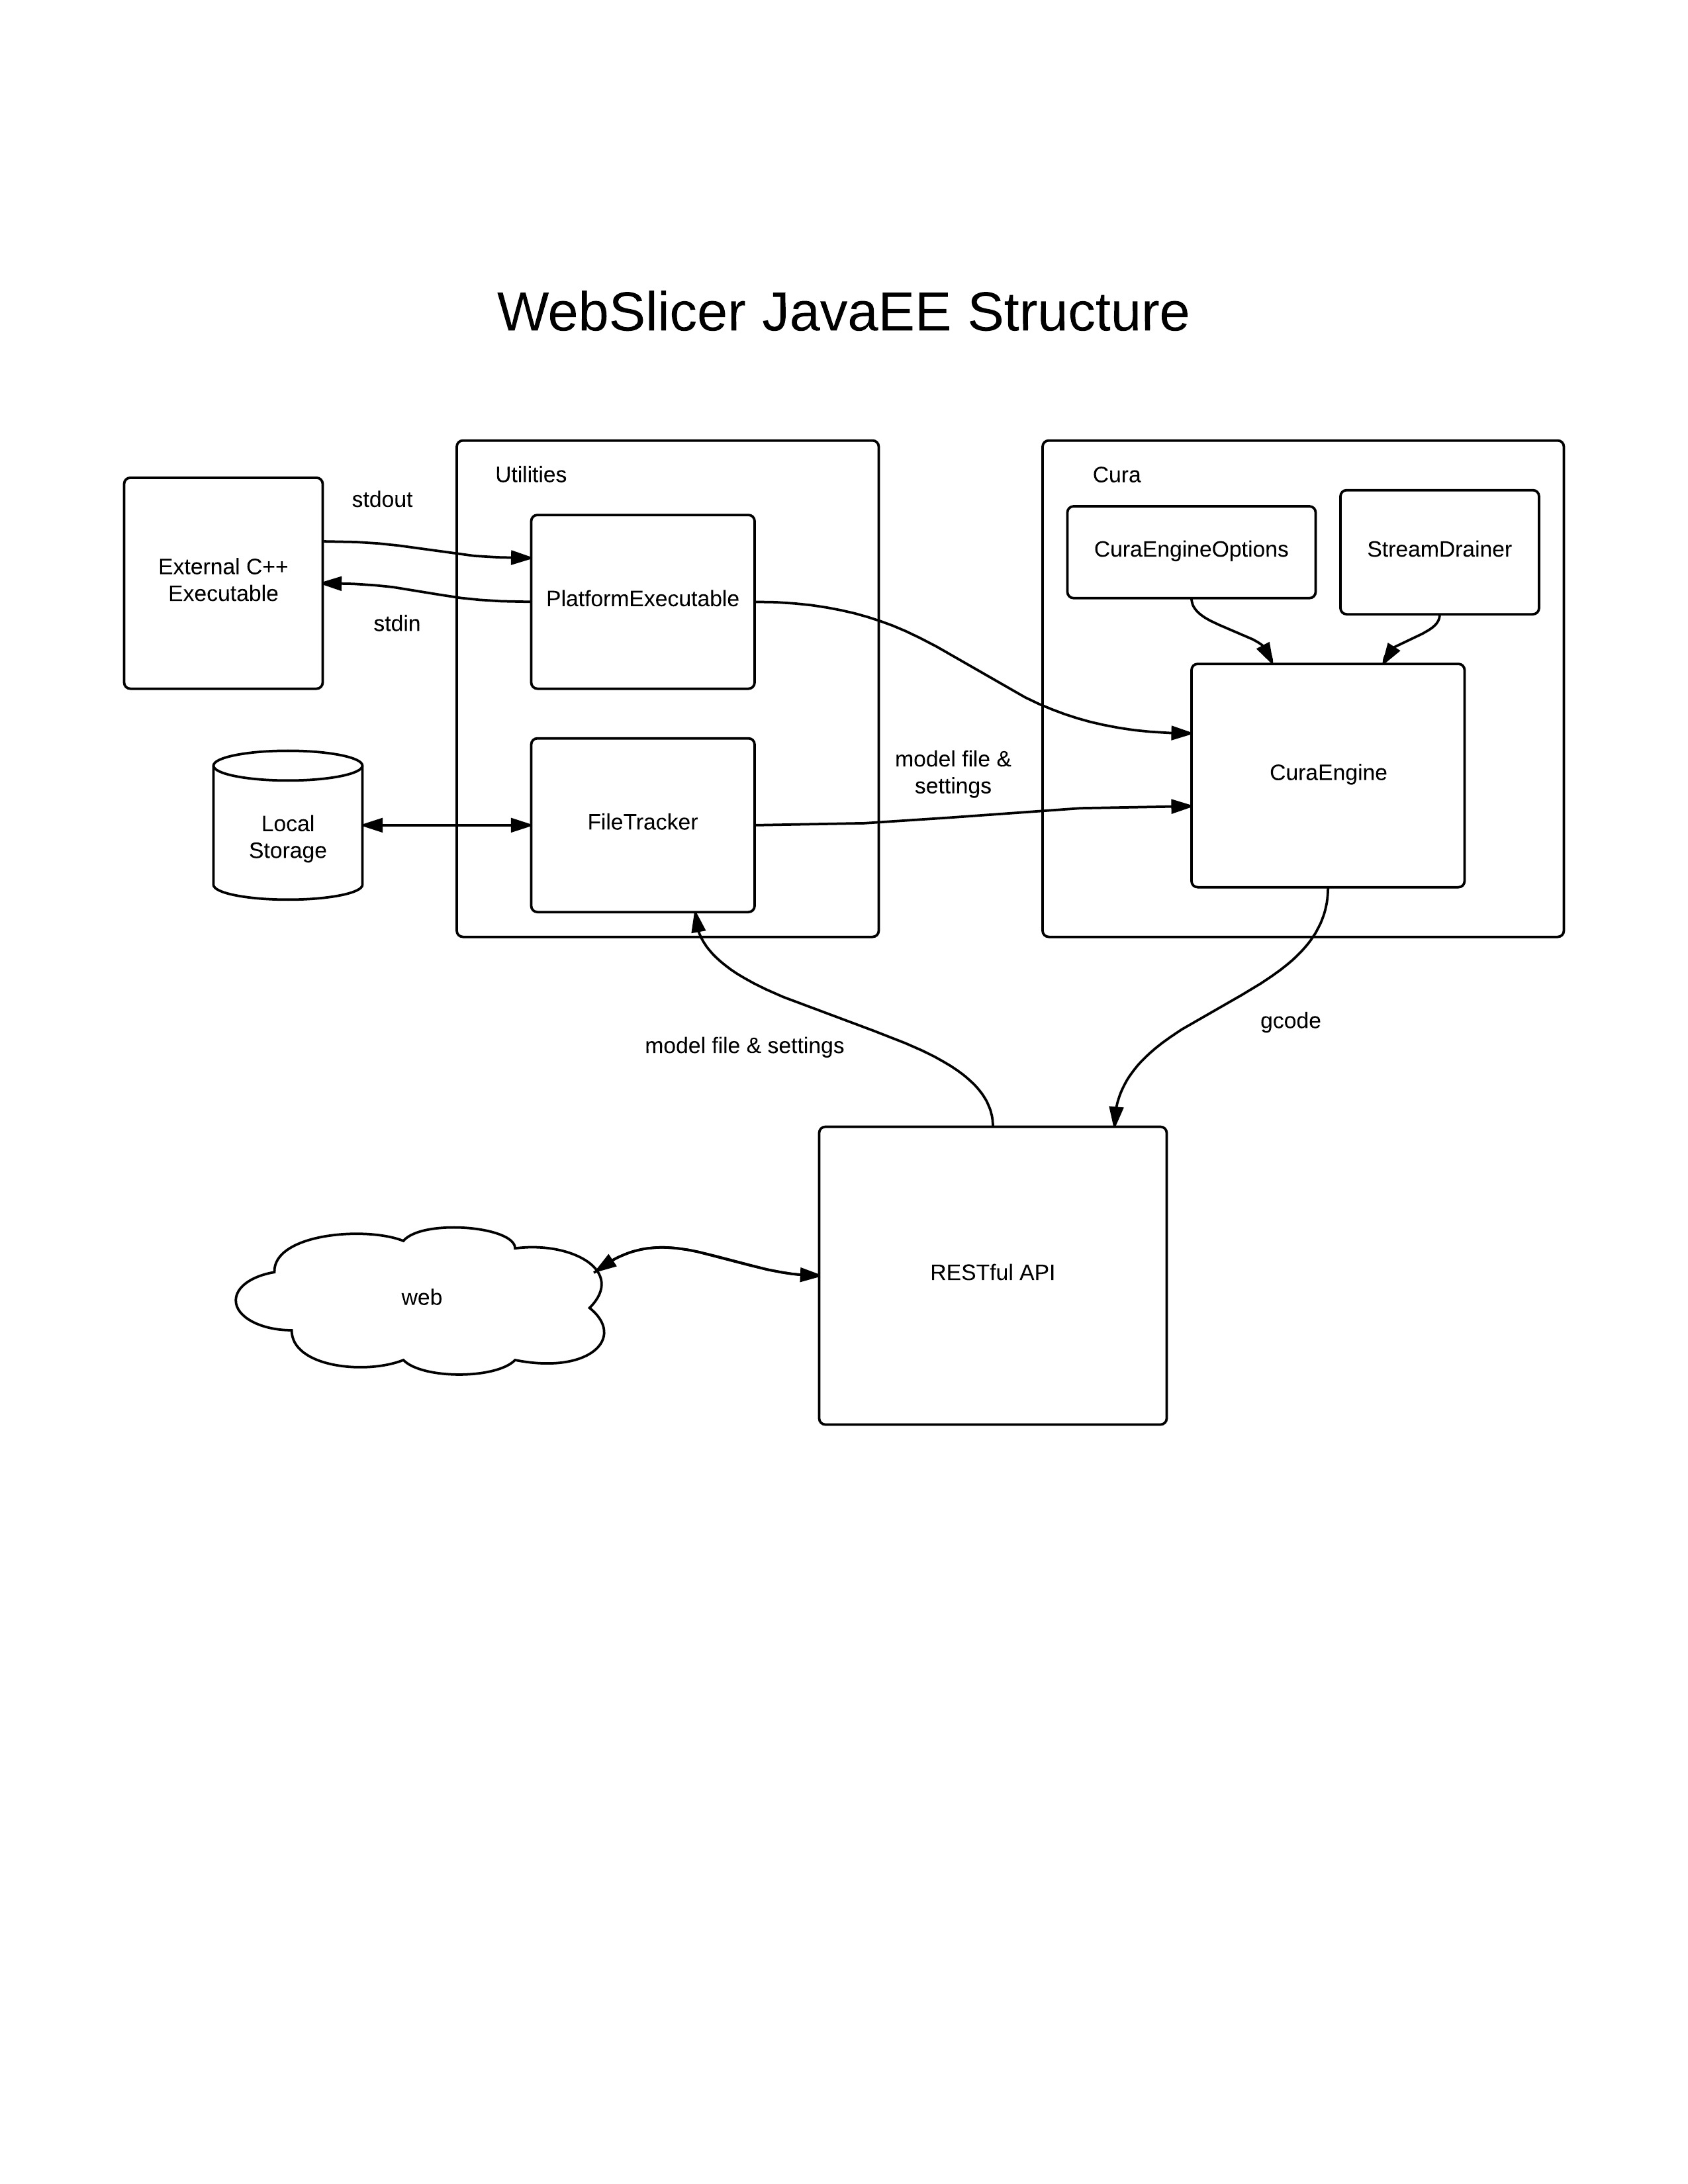
\includegraphics[width=\linewidth]{Server-Side-Structure}
  \caption{The structure of the server side of WebSlicer}
  \label{fig:server-side-structure}
\end{figure}

\section{JavaEE 7}
% talk about why its awesome and how i structured my code.
% give enough background to exalain what is needed
% maven archetype stuff
% 
\section{ProcessBuilder}
% ignore CuraEngine and talk only about how ProcessBuilder works with diagrams
\section{CuraEngine Integration}
% how it works with ProcessBuilder
\section{REST API}
% my REST API and the reason that I structured it the way I did

\section{Key Challenges}
\subsection{ProcessBuilder Deadlock}
\paragraph{}

\subsection{FileTracker Revamp}
\paragraph{}
%copy/pasta this from wordpress blog
%make updated flowchart for this.

\section{Issues \& Known Bugs}
%unable to import existing files


